\documentclass[a4paper, itemph]{oblivoir}
\setmainhangulfont{NANUMMYEONGJO.TTF}[BoldFont={NANUMMYEONGJOEXTRABOLD.TTF}]
\usepackage[english]{babel}
\usepackage[utf8x]{inputenc}
\usepackage[T1]{fontenc}
%% Sets page size and margins
\usepackage[a4paper,top=3cm,bottom=2cm,left=3cm,right=3cm,marginparwidth=2cm]{geometry}

\usepackage{indentfirst}

%% Useful packages
\usepackage{amsfonts}
\usepackage{amsmath, mathtools}
\usepackage{graphicx}
\usepackage{subcaption}
\usepackage[colorinlistoftodos]{todonotes}
\usepackage{amssymb}
\usepackage{amsthm}
\usepackage{tikz}

%Extravaganza
\newtheorem{thm}{Theorem}[subsection]
\newtheorem{lem}{Lemma}[subsection]
\newtheorem{cor}{Corollary}[subsection]
\newcommand{\overbar}[1]{\mkern 1.5mu\overline{\mkern-1.5mu#1\mkern-1.5mu}\mkern 1.5mu}
\theoremstyle{definition}
\newtheorem{defn}{Definition}[subsection]
\newtheorem{rem}{Remark}[subsection]

\begin{document}
\title{기초전자회로 및 실험: Lab \#04}
\author{서울대학교 전기$\cdot$정보공학부 2018-12602 이준협}
\maketitle

\section{Determining the Collector and Emitter}
\begin{figure}[htb]
    \centering
    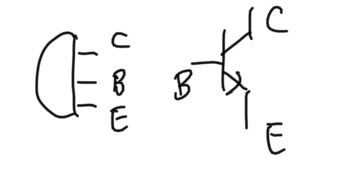
\includegraphics[width=0.3\linewidth]{cbe.JPG}
    \caption{The determined nodes. When the transistor is placed so that the curved part looks to the left, the nodes are placed in the order of C, B, and E.}
\end{figure}

The collector and the emitter were determined by treating the PN junctions between the collector and the base/emitter and the base as diodes. That is, when we apply a constant voltage $V_{BE}>0$/$V_{BC}>0$ while leaving the collector/emitter open and measure the current $I_E/I_C$, we expect $I_C>I_E$ and therefore the junction with the higher current was identified as the emitter-base junction. This is because the doping concentration $N_{D,E}$ is much higher than $N_{D,C}$, therefore the minority carrier density at the edge of the depletion region is much lower at the emitter side.
\begin{table}[htb]
    \centering
    \begin{tabular}{c|c|c}
        $V_{BE}=V_{BC}[mV]$ & $I_E[mA]$ & $I_C[mA]$\\
        \hline
        570 & 0.056 & 0.079
    \end{tabular}
    \caption{The emitter and collector currents when the PN junctions between each area and the base are treated as diodes.}
\end{table}

Whether the emitter and the collector were determined properly was also confirmed by checking the current gain in section 2. If the emitter and collector were not determined properly, the current gain would have been insignificant.
\section{Common Emitter Properties}
To extract the thermal voltage, $V_{BE}=V_{CE}$ is varied(edge of saturation) and the collector current is measured. Then the natural logarithm of the current is plotted against the base voltage. The slope must be $\dfrac{1}{V_T}$.
\begin{table}[htb]
    \centering
    \begin{tabular}{c|c|c|c|c|c}
        $V_{BE}[mV]$ & 579 & 602 & 634 & 650 & 670 \\
         \hline
         $I_C[mA]$ & 0.204 & 0.466 & 1.668 & 3.06 & 6.38
    \end{tabular}
    \caption{Collector currents when the transistor is turned on.}
\end{table}

\begin{figure}[htb]
    \centering
    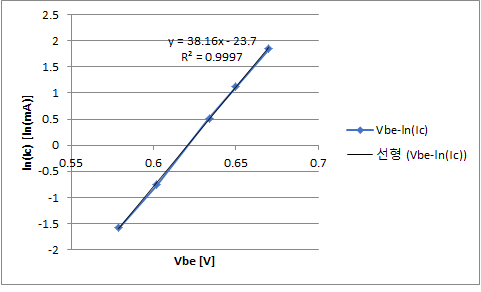
\includegraphics[width=0.5\linewidth]{V_T.png}
    \caption{$\ln{I_C}-V_{BE}$ plot to determine $V_T$.}
\end{figure}
The linear plot between the logarithm of the current and the base voltage is in figure 2, and since the slope is 38.16, the thermal voltage is $\dfrac{1}{38.16}=0.0262[V]=26.2[mV]$, which agrees with theory. That is, the current increases exponentially with respect to the base-emitter forward bias, and the thermal voltage is of the same order with $\dfrac{kT}{q}$.
\begin{figure}[htb]
    \centering
    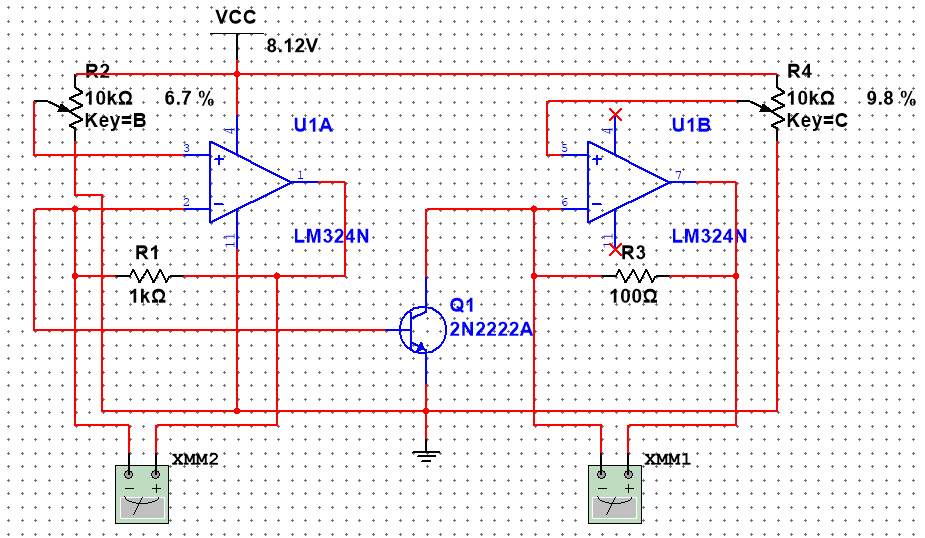
\includegraphics[width=0.5\linewidth]{CE_circuit.PNG}
    \caption{The circuit used to measure the base and collector current. The voltage follower is used to fix the base and collector voltage, and the currents are measured from the voltages across the $100[\Omega]$ and $1000[\Omega]$ resistances. The resistances are variable resistors that were controlled to fit the ideal value, and $V_{DD}=8.12[V]$.}
\end{figure}

Next, the variation of the collector current with respect to the collector voltage was measured with $V_{BE}$ fixed at $602/634/650[mV]$, using the circuit in figure 3.
\begin{figure}[htb]
    \centering
    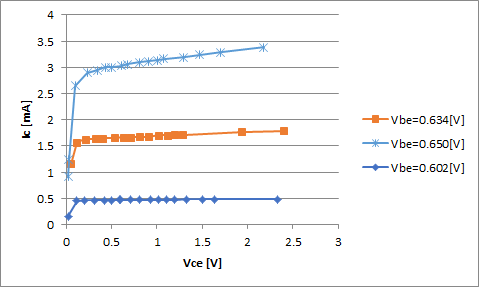
\includegraphics[width=0.5\linewidth]{CE.png}
    \caption{The $I_C-V_{CE}$ graph of the circuit in the common emitter configuration.}
\end{figure}

The collector current was measured from $V_{CE}\approx0[V]$ until $V_{CE}\approx1[V]$, when the voltage was incremented by $0.1[V]$. To calculate the Early voltage, few more points were measured until $V_{CE}\approx 2.5[V]$. As expected, the collector current rises abruptly as $V_{CE}$ rises, since the minority charge carrier density near the base-collector junction falls exponentially as the base-collector reverse bias increases. We can calculate the $\beta$ values from $I_C/I_B$ when $V_{CE}>V_{BE}$. If we use the mean of $I_C/I_B$ as $\beta$, we get $\beta=157.4/173.9/174.5$ for $V_{BE}=0.602/0.634/0.650[V]$. In other words, $\alpha=0.99369/0.99428/0.99430$. The raw data is shown in figure 5.
\begin{figure}[htb]
    \centering
    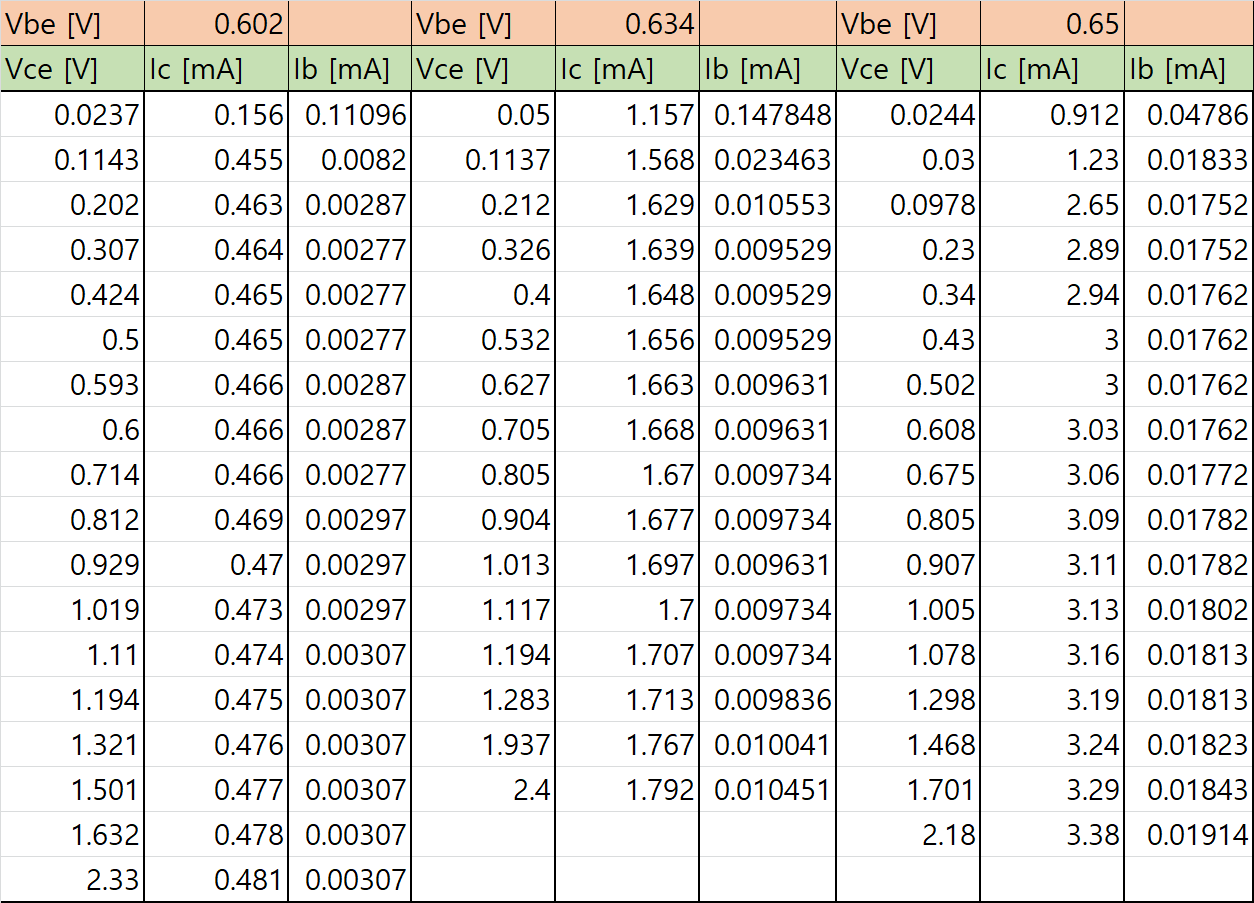
\includegraphics[width=0.5\linewidth]{CE_data.png}
    \caption{The data used to calculate $\beta$.}
\end{figure}

The fact that $\beta$ increases as collector current increases fits with theory. According to [1], at low current conditions when the collector current varies with $\exp{\dfrac{qV_{BE}}{kT}}$, as is the case in this experiment, the surface leakage current at the base is significant enough to lower the efficiency of $V_{BE}$ in increasing the base current. That is, $I_B$ varies with $\exp{\dfrac{qV_{BE}}{mkT}}(m>1)$. Then $I_C/I_B$ must increase as $V_{BE}$ increase, so $\beta$ is calculated to be increasing. The measurements of $\beta$ fits in with the $h_{FE}$ measurement performed by the multimeter, as the multimeter measured $h_{FE}=200$.

Next, the early voltage was extrapolated from fitting the collector current in the forward active region by a linear model and calculating the $x-$intercept.

\begin{figure}[htb]
    \centering
    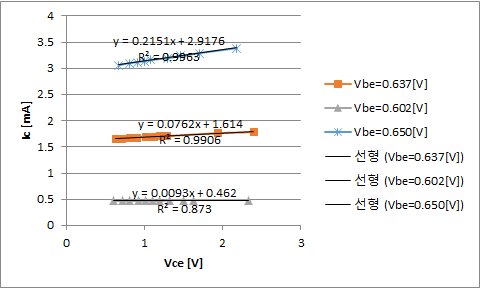
\includegraphics[width=0.5\linewidth]{early.png}
    \caption{Linear fit of the collector current in the forward active region as to extrapolate $V_A$.}
\end{figure}
\begin{table}[htb]
    \centering
    \begin{tabular}{c|c|c|c|c}
        $V_{BE}[mV]$ & $V_A[V]$ & $r_o[k\Omega]$ & $g_m[S]$ & $r_\pi[\Omega]$\\
        \hline
        602 & 49.68 & 107.5 & 0.0178 & 8850\\
        \hline
        634 & 21.18 & 13.12 & 0.0635 & 2740\\
        \hline
        650 & 13.56 & 4.649 & 0.117 & 1494
    \end{tabular}
    \caption{$V_A$ and $r_o$ are extracted directly from the linear plot. $V_A$ is the absolute value of the $x-$intercept, and $r_o$ is 1/(slope). $g_m$ and $r_\pi$ are calculated by $g_m=I_C/V_T$, $r_\pi=\beta/g_m$, when $I_C$ is the current at the edge of saturation.}
\end{table}

As can be seen from table 3, $V_A$ is roughly between $15[V]$ and $150[V]$, which is the range of the Early voltage expected in [1]. However, what is strange is that the Early voltage varied drastically according to the variation in collector current. That can be explained by the effect of BJT self-heating. Since the BJT is highly sensitive to temperature change and its current changes exponentially according to temperature, more current, leading to more Ohmic power dissipation and higher temperature, forcibly increases the slope in figure 6 to something that depends not on $\exp{\dfrac{qV_{BE}}{kT}}$($\because I_C=I_S\exp{\dfrac{qV_{BE}}{kT}}(1+\dfrac{V_{CE}}{V_A})$, so the slope is $\dfrac{I_S}{V_A}\exp{\dfrac{qV_{BE}}{kT}}\propto \exp{\dfrac{qV_{BE}}{kT}}$) but on a higher order term. What supports this argument is the fact that the measurements of collector current when $V_{BE}$ is constant is even more sensitive to temperature change. Figure 7(which is Fig. 2 in [2]) illustrates this.
\begin{figure}[htb]
    \centering
    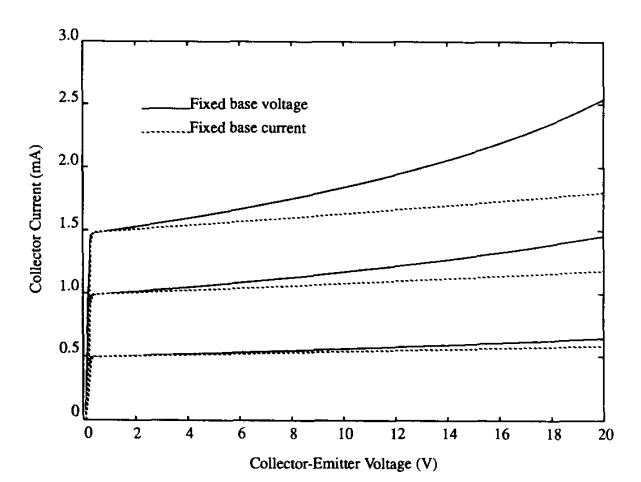
\includegraphics[width=0.5\linewidth]{self heating.PNG}
    \caption{Increase of slope of the $I_C-V_{CE}$ curve due to BJT self-heating. Figure from [2].}
\end{figure}

It would've been more appropriate if there was a current source available that could provide currents in the $\mu A$ region, then that current source would have been useful in fixing the base current.
\section{Conclusion}
Although we could only provide constant base voltage, the exponential characteristic of $I_C$ with respect to base voltage and the Early effect could be well-confirmed, and the small-signal characteristics of the BJT were derived from such observations.
\begin{thebibliography}{}

\bibitem{1} S. M. Sze and K. K. Ng, \textit{Physics of Semiconductor Devices}, 4th ed. Hoboken, NJ: Wiley, 2015, pp. 243-292.
\bibitem{2} R. M. Fox, S. Lee, and D. T. Zweidinger , “The Effects of BJT Self-Heating on Circuit Behavior,” \textit{IEEE Journal of Solid-State Circuits}, vol. 28, no. 6, pp. 678–685, June 1993.

\end{thebibliography}

\end{document}
